\chapter{Background}

Parton distribution functions (PDFs) bridge the gap between short and long range physics, allowing perturbative Quantum Chromodynamics (QCD) to be applied at the hadronic scale. They embody the incalculable strongly coupled dynamics, and are determined by a comparison of perturbative theory with experiment. Once determined, their form is process-independent and so they can be re-deployed in future calculations. 

This section provides some background to PDFs neccesary for understanding the remainder of this thesis. It is divided in to two main parts, being the necessary physics and the necessary methodology of PDF determination.

To review the physics, we begin by looking at the process of deep inelastic scattering (DIS), and how the na\"ive parton model was developed to explain these experimental observations. Next we look at this in the context of QCD, see how PDFs fit into the picture, and how they evolve with the scale of the physics. Finally we briefly touch on hadron-hadron collisions, which along with DIS constitute the bulk of the processes in modern PDF fits.

To review the methodology we consider the NNPDF fitting strategy, explaining how theory and experiment are used together with neural networks to determine PDFs.

\subsection{Deep inelastic scattering}

Deep inelastic scattering (DIS) experiments were some of the earliest high energy physics experiments to involve hadrons. The set-up constitutes a beam of charged leptons scattering off a stationary hadronic target, for example electrons incident on protons, as shown in Fig. \ref{fig:dis}. In the deep inelastic regime, there is a large momentum transfer, $q=k-k'$, mediated by a virtual photon. The proton, with initial momentum $P$, fragments into some hadronic state $X$, and the electron starts with energy $E$ and momentum $k$ and ends with energy $E'$ and momentum $k'$. The momentum transfer is large enough that the masses of the proton and electron can be neglected. 

\begin{figure}[H]
\label{fig:dis}
\centering
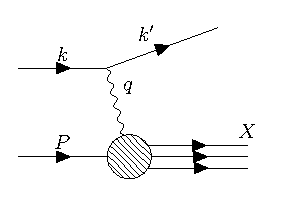
\includegraphics[width=0.7\textwidth]{../diagrams/disdiag.pdf}
\caption{Deep inelastic scattering}
\end{figure}

It is customary to define some useful variables for help in the analysis, listed in the table below.
\begin{table}[H]
\centering
\begin{tabular}{l|l|l}
  Variable & Definition & Interpretation   \\
 \hline
  $Q^2$ & $- q^2 = -(k-k')^2$   & momentum transfer    \\
  $\nu$ & $p \cdot q = M(E'-E)$ & energy transfer  \\
  $x$   & $\frac{Q^2}{2\nu}$    & scaling parameter \\
  $y$   & $\frac{q \cdot p}{k \cdot p} = 1 - \frac{E'}{E}$ & inelasticity $\epsilon$ (0,1)
\end{tabular}
\end{table}
\subsection{The parton model}
\subsection{Quantum Chromodynamics (QCD)}
\subsection{The QCD improved parton model and factorisation}
\subsection{Evolution and the DGLAP equation}
\subsection{Hadroproduction}

In the Standard Model of particle physics, the strong force is responsible for short range interactions
which bind together quarks. The theory of the strong force is known as Quantum Chromodynamics (QCD),
with corresponding Lagrangian

\beq
  \mathcal{L}_{QCD} = - \frac{1}{4} F_{\alpha \beta}^A F_A^{\alpha \beta} + \sum_{flavours} \bar{q}_a(i \slashed{D}-m)_{ab}q_b,
\eeq
where the field strength tensor is given by
\beq
  F_{\alpha \beta}^A = \bigg[ \partial_\alpha \mathcal{A}_\beta^A - \partial_\beta \mathcal{A}_\alpha^A
    - g f^{ABC} \mathcal{A}_\alpha^B \mathcal{A}_\beta^C \bigg]
\eeq
(ignoring gauge-fixing and ghost terms) \cite{ob:ellis}. Upper case Latin letters label
\textit{colour}, lower case Latin letters label \textit{flavour} and lower case Greek letters
run over dimensions. The first term in the Lagrangian arises from self-interacting gluons,
$\mathcal{A}$, and the second term comes from quarks, $q$, which obey the Dirac equation.

Hadroproduction at the LHC consists of processes like $pp \to X$, where $p$ is a proton and $X$ is some 
final hadronic state.
This means experimental measurements are typically of some observable based on the cross-sections $\sigma_{pp\to X}$.
Theoretical predictions are usually performed at the partonic level, for interactions between partons $a$
and $b$, \textit{i.e.} $\hat{\sigma}_{ab \to X}$. The convention here is that hats apply to partonic variables and no-hats apply to hadronic variables. Factorisation theorems \cite{jr:collins} allow the hadronic cross
section to be expressed as a convolution of the partonic cross sections with relevant PDFs, $f$:

\beq
  \sigma_{pp \to X} (s, M_X^2) = \sum_{a,b} \int dx_1 dx_2\ f_a(x, \mu_F^2)\ f_b (x_2, \mu_F^2)\ \hat{\sigma}_{ab \to X} (x_1x_2s, M_X^2, \mu_R^2, \mu_F^2)
\label{factorisation}
\eeq  
  
where $x$ is the momentum fraction of the proton associated with each parton, $s$ is the proton
centre-of-mass frame energy and $M_X$ is the invariant mass of the final state $X$. 

PDFs depend on the scale, $\mu_F$, at which the factorisation is applied. However, this is an artificially
introduced scale so observables such as $\sigma_{pp \to X}$ must be independent of it. This observation
leads to a series of coupled partial differential ``renormalisation group'' equations relating PDFs at
different scales known
as the Dokshitzer-Gribov-Lipatov-Altarelli-Parisi (DGLAP)
equations~\cite{jr:altarelli}\cite{jr:dokshitzer}\cite{jr:gribov}:

\beq
  \mu_F \frac{d}{d\mu_F} f_i (y, \mu_F^2) = \sum_j \int_z^1 \frac{dz}{z} \mathcal{P}_{ij}\bigg(
  \frac{y}{z}, \alpha_s \bigg) f_j (z, \mu_F^2).
\label{eq:DGLAP}
\eeq

These show that the scale dependence of a given parton's PDF depends on all the other partons' PDFs through
``splitting functions'' $\mathcal{P}_{ij}$, which in turn depend on the strong coupling constant $\alpha_s$.

Although PDFs may seem at first sight to be totally unknown there are some theoretical observations which
we can use to constrain their form.
These are known as the ``sum rules''~\cite{ob:ellis}. Intuitively, adding up all the momenta of the partons must equal the
momentum of the proton. This enforces the condition

\beq
  \int_0^1 dx \sum_i x f_i(x,Q^2) = 1.
\eeq

The other thing we know about the
proton is that it is made up of two up and one down (and no strange)
``valence'' quarks. Any other quarks must be pair-produced from the sea, and
therefore come with an antiquark of the same flavour. So we can normalise the PDFs using the expressions: 

\begin{subequations}
 \beq
   \int_0^1 dx \big( f_u - f_{\bar{u}} \big) = 2;
 \eeq
 \beq
   \int_0^1 dx \big( f_d - f_{\bar{d}} \big) = 1;
 \eeq
 \beq
   \int_0^1 dx \big( f_s - f_{\bar{s}} \big) = 0.
 \eeq
\end{subequations}

Note that these conditions require that the PDFs are integrable. 


\section{Determining PDFs}
\subsection{Experimental uncertainties}

Experimental uncertainties are implemented via a \textit{covaraince matrix} which links vectors of
data points. This encapsulates the total breakdown of errors, $\rho$, and can be constructed: 
\beq
  \sigma_{ij} = \delta_{ij}\rho_i^{uncorr}\rho_j^{uncorr} + \sum_a^{+}\rho_{i,a}\rho_{j,a} +
  \bigg( \sum_m^{\times}\rho_{i,m}\rho_{j,m} \bigg) T^0_i T^0_j.
\label{eq:expcov}
\eeq
The notation $\sum^{+}$ indicates a sum over additive systematics and $\sum^\times$ over
multiplicative systematics (more on this below).

Here the uncorrelated statistical uncertainties appear down the diagonal, but correlated
systematic uncertainties can also appear on the off-diagonals. Correlated uncertaintes include
those which link multiple data points, for example systematic uncertainties from a particular
detector which will affect all of its data in a similar way.

Systematic uncertainties further divide into two types, ``additive'' and ``multiplicative''.
Additive systematics are perhaps a more familiar type of error, and are independent of the
datapoint values themselves. On the other hand,  multiplicative systematics depend on the measured values. In the context of particle physics 
experiments, a common example is total detector luminosity. This is because recorded cross
sections are dependent on the luminosity of the detector; a higher luminosity means more
collisions will take place so the measured cross section will be greater.

The covariance matrix is used in two places during the fit; the generation of pseudodata and calculation
of $\chi^2$.

\subsection{Pseudodata}
\subsection{NNPDF fitting strategy}

There are a number of groups currently active in carrying out PDF fits and these include MSTW~\cite{Martin:2009bu}, CTEQ~\cite{Dulat:2015mca}, NNPDF~\cite{Ball:2017nwa}, HERAPDF/xFitter~\cite{CooperSarkar:2011aa} and ABM~\cite{Alekhin:2013nda}.

The work in this thesis has been carried out in the framework developed by the NNPDF collaboration, so we will henceforth concentrate on this fitting strategy. There are two main features which differ from other fitting collaborations'~\cite{Forte:2002fg}. These are:

\begin{figure}
\centering
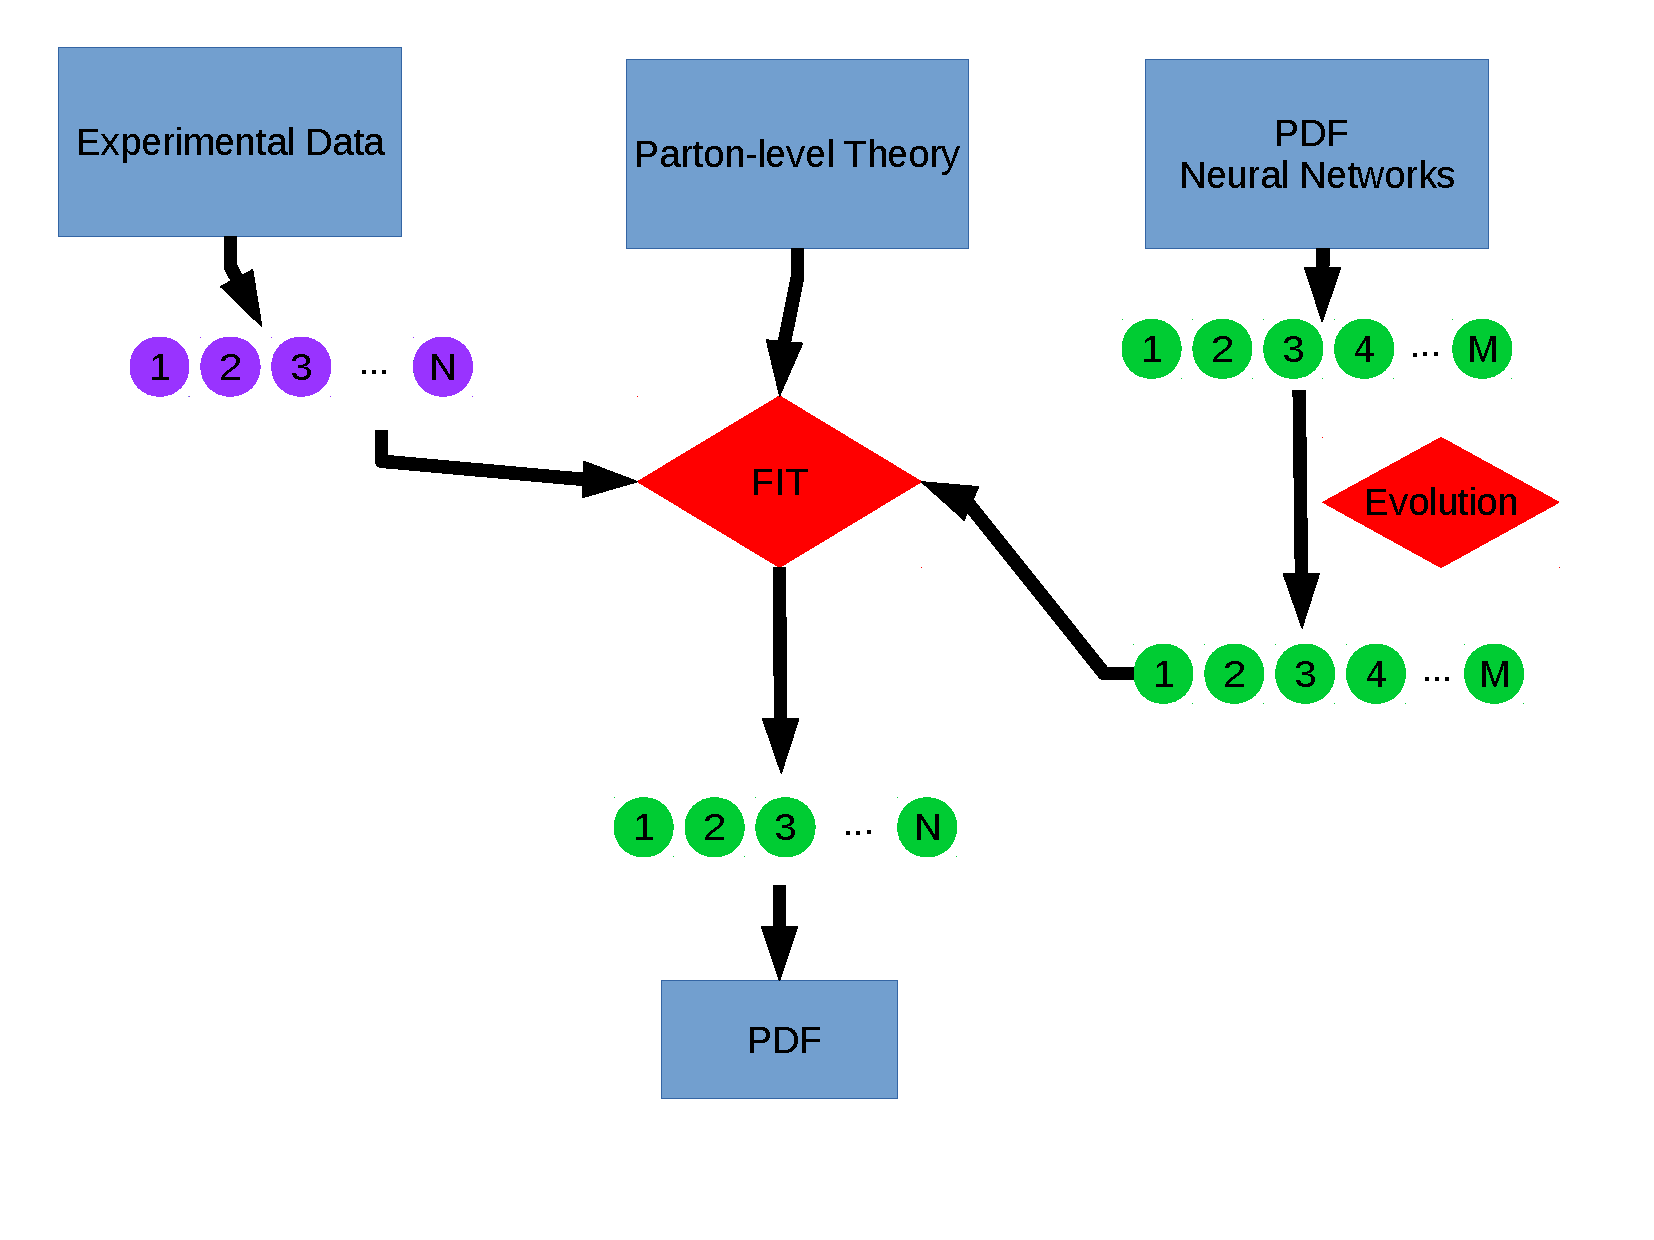
\includegraphics[width=0.8\textwidth]{background/general_strategy_diagram.pdf}
\caption{NNPDF general strategy.}
\label{flowchart}
\end{figure}

\begin{enumerate}
\item  the use of Monte Carlo rather than Hessian approach to error analysis;
    \item  fitting using artificial neural networks.
\end{enumerate}

Fig. \ref{flowchart} outlines the NNPDF general strategy. Experimental data is converted into an ensemble of $N$ artificial Monte Carlo replicas or \textit{pseudodata}. These are randomly generated in accordance with multi-Gaussian distributions centred around each data point, with variance given by the experimental uncertainty (see Fig. \ref{MC}). Each Monte Carlo replica contains the same number of data points as the original experimental measurements. Given enough replicas, the Monte Carlo set contains complete experimental information; the experimental central value can be retrieved by taking the mean, and the experimental variance is the variance calculated over the replicas. 

\begin{figure}
\centering
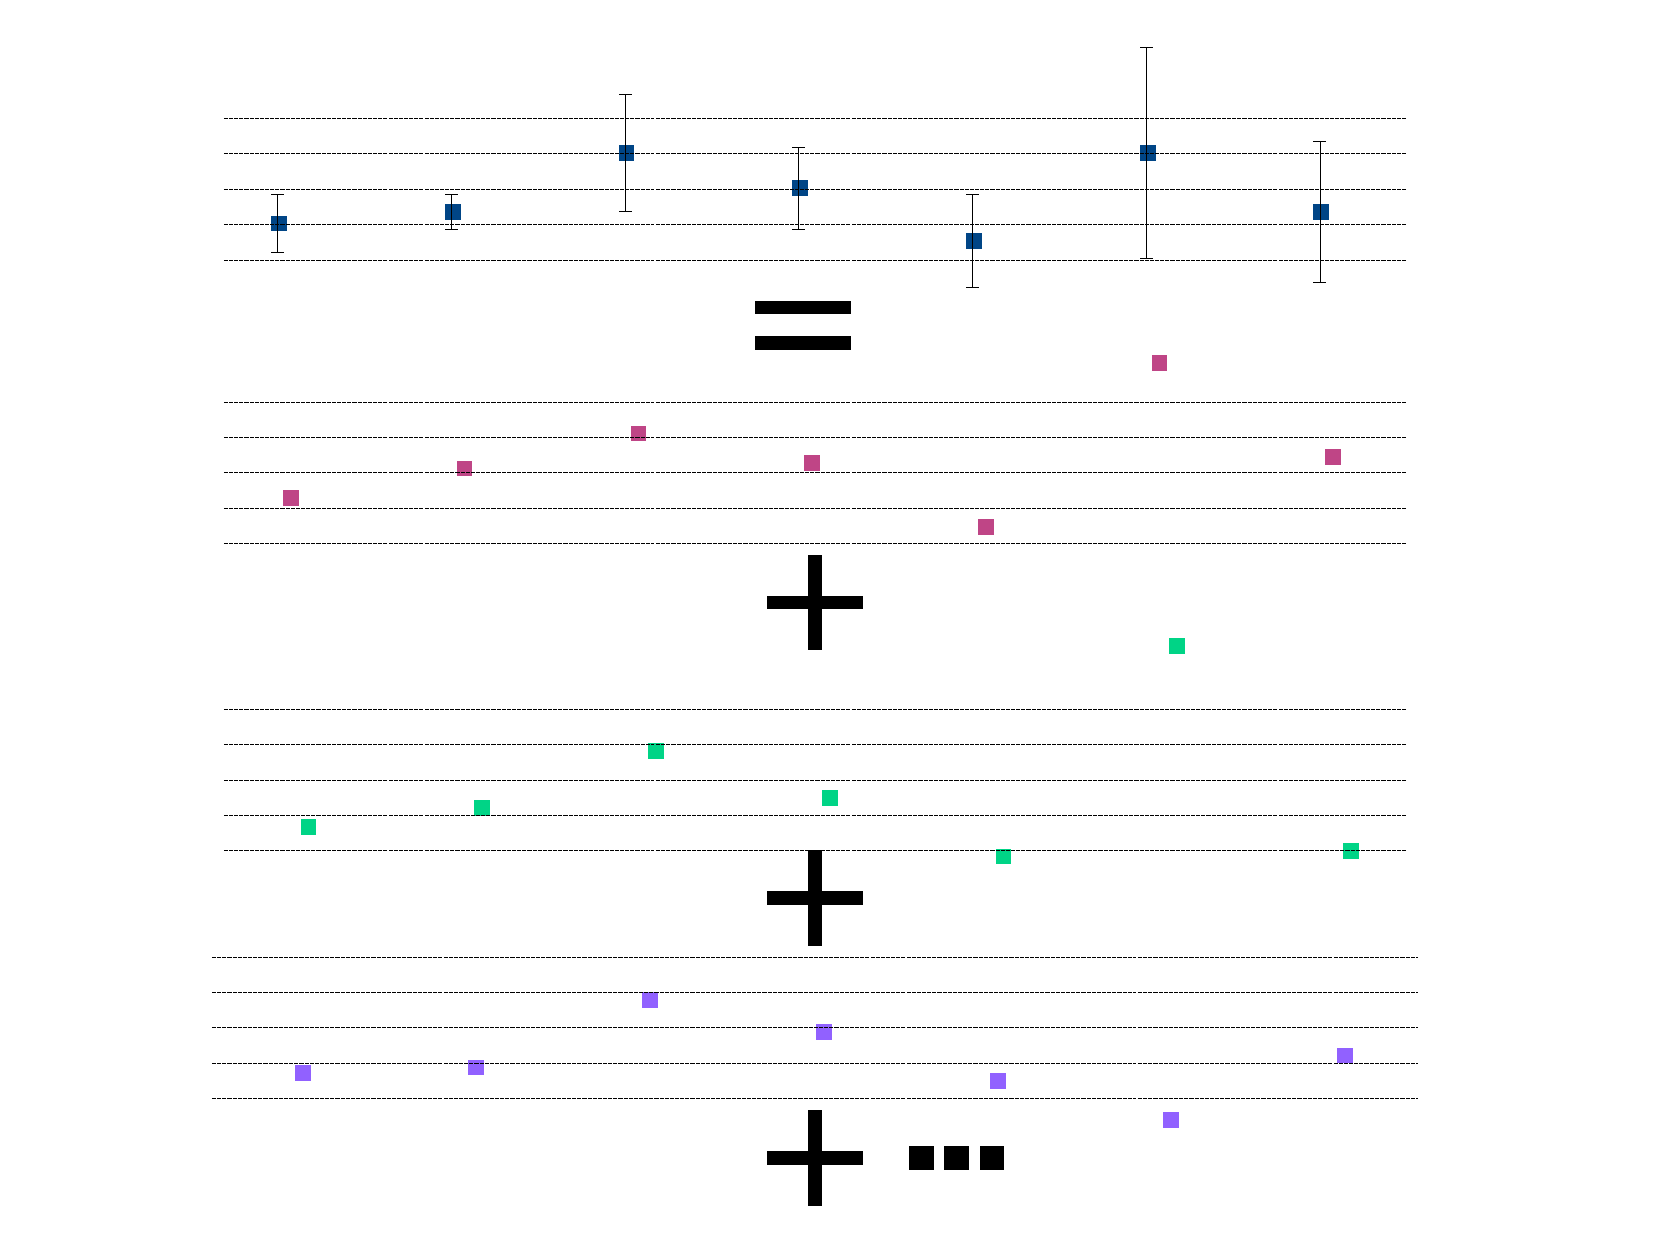
\includegraphics[width=0.7\textwidth]{background/monte_carlo.pdf}
\caption{Generation of Monte Carlo replicas of pseudodata using a Gaussian probability density
  function which has the same mean and variance as the experimental data. This means that the
  mean and variance of the replicas can reproduce those of the experimental data arbitrarily
  closely, given enough replicas.}
\label{MC}
\end{figure}


NNPDF uses a variety of experimental data from a number of particle colliders. These are observables such as cross sections, differential cross sections and structure functions. Fig. \ref{data} is a plot of the $(x,Q^2)$ range spanned by the datasets in the latest NNPDF3.1~\cite{Ball:2017nwa} release. Here $x$ and $Q$ are Bj\"orken variables corresponding to the parton momentum fraction and the energy scale of the process. The majority of the data are from DIS.

\begin{figure}
\centering
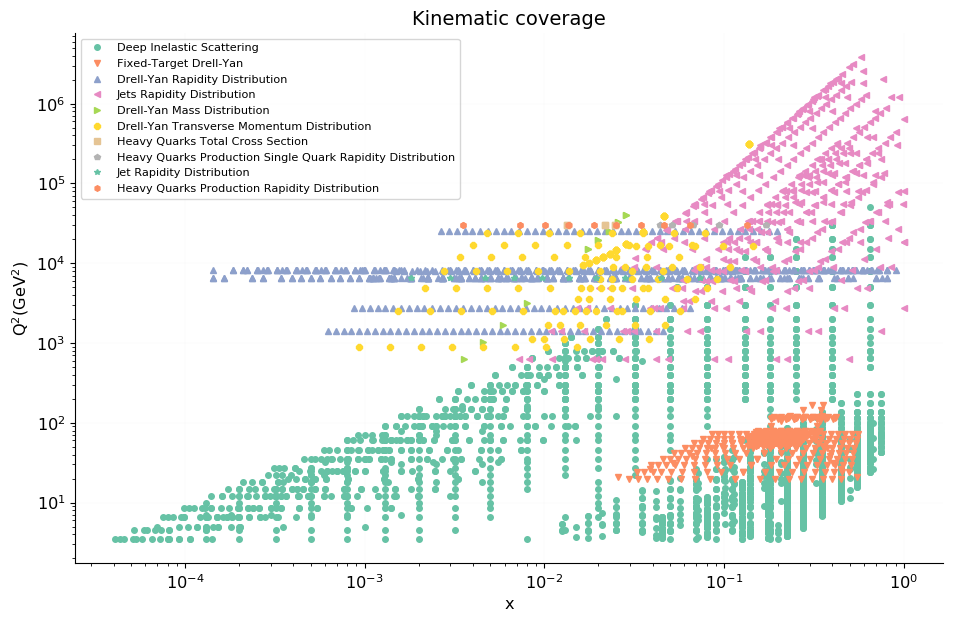
\includegraphics[width=15cm]{background/NNPDF31_nlo_as_0118_1000_markers0_fitcontext_plot_xq2.png}
\caption{Plot of the $(x,Q^2)$ range spanned by data included in the latest NNPDF3.1 NLO fit.}
\label{data}
\end{figure}

Theoretical predictions of parton-level observables are computed using external codes such as \texttt{MCFM}~\cite{jr:mcfm}, \texttt{DYNNLO}~\cite{Catani:2009sm}, \texttt{FEWZ}~\cite{Gavin:2010az} and \texttt{NLOjet++}~\cite{Catani:1996vz}. These are converted to higher orders as necessary using QCD and electroweak correction (``$k$'') factors. They are then combined with DGLAP evolution kernels, which evolve PDFs from an initial reference energy scale to the energy scale of each experiment using the DGLAP equations (Eqn. \ref{eq:DGLAP}). 

Next, $M$ independent artificial neural networks are generated. These are combined with the partonic theory and compared to the experiments in a global fit. Here each pseudodata set is fitted against all the neural networks, which learn the functional form of the PDF.  The best fit is determined based on some suitable figure of merit such as $\chi^2$ value between the experimental observables and the theoretical observables calculated using the current iteration of PDFs. 

In order to prevent overlearning, where the neural network also fits random fluctuations in the data, the pseudodata are divided into two sets, one for training and one for validation. At each step in the fit the $\chi^2$ is computed for both sets, but minimisation is based only on the training set. When the $\chi^2$ of the validation set stops decreasing, this signifies that overlearning has begun so any subsequent versions of the PDF can be discarded. 

\begin{figure}
  \begin{minipage}[c]{0.40\textwidth}
    \caption{
       The Monte Carlo replicas for the down valence quark PDF NNPDF3.1 at NLO. The scale is Q = 10 GeV
    } \label{replicas}
  \end{minipage}
  \begin{minipage}[c]{0.55\textwidth}
    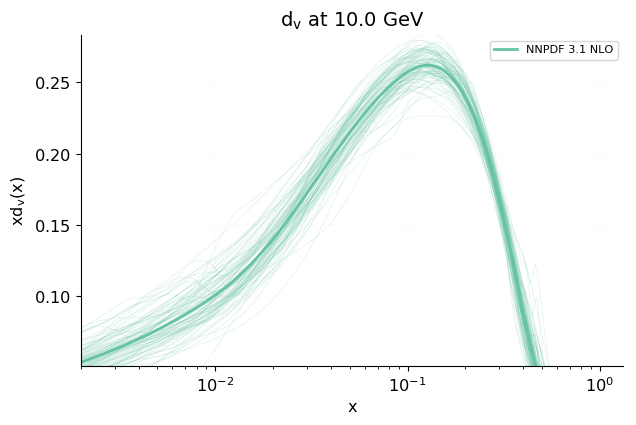
\includegraphics[width=\textwidth]{background/Qs0_NNPDF31NLO_plot_pdfreplicas_d_v.png}
  \end{minipage}\hfill
\end{figure}
The whole fitting process produces $N$ ``best fit'' neural networks, which act as a Monte Carlo parametrisation of the PDF (for example Fig. \ref{replicas}). This means that the PDF and its error can be extracted by taking the mean and standard deviation. The final PDFs are made publicly available on the LHAPDF \cite{Buckley:2014ana} website (\texttt{https://lhapdf.hepforge.org/}).
\subsection{Neural Networks}

Inspired by how the brain processes information, neural networks are composed of a collection of nodes
known as \textit{neurones}, connected together in various ways. They are trained by example, so
have the capability to learn a PDF's functional form given a set of data. The layout consists
of input layers, hidden layers and output layers, as shown in Fig. \ref{nnet}. In a feed-forward
neural network, information can only be passed in one direction through the layers (from 
input to output). Here, the output
of a neurone in the $l^{th}$ layer is given by
\beq
  \xi_i^{(l)} = g \bigg( \sum_j^{inputs} \omega_{ij}^{(l)} \xi_j^{(l-1)} + \theta_i^{(l)} \bigg)
\eeq
where the $\omega$s and $\theta$s are ``weights'' and ``thresholds''; parameters to be minimised
with respect to.  $g$ is an ``activation function'' which is set to
\beq
  g(a) =
\begin{cases}
 \frac{1}{1 + e^{-a}} &\text{for hidden layers}\\
  a &\text{for output layer}.
\end{cases}
\eeq

\subsection{Parametrisation}
\subsection{Preprocessing}
PDFs at a given energy scale can be evolved to any other scale using the DGLAP equations 
(Eqn. \ref{eq:DGLAP}).
In order to aid the fitting process, the PDFs undergo \textit{preprocessing};
they are parametrised as:

\beq
  f_i(x) = A_i x^{-\alpha_i} (1-x)^{\beta_i} N_i(x)
\eeq

\begin{wrapfigure}{L}{0.5\textwidth}
\centering
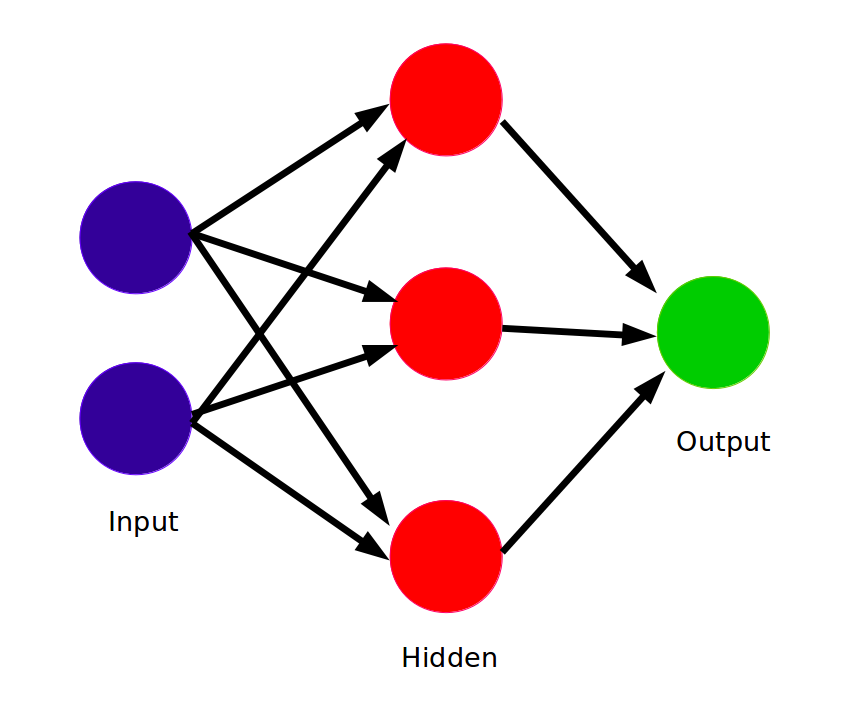
\includegraphics[width=0.48\textwidth]{background/nnet.png}
\caption{Schematic depiction of an artificial neural network.}
\label{nnet}
\end{wrapfigure}
where $A_i$ are coefficients set by the sum rules (see earlier) and $\alpha_i$ and $\beta_i$ are parameters
to be fitted. $N_i(x)$ are artificial neural networks. This form is chosen to force the 
PDFs to 0 at large $x$. 
\subsection{Positivity}
\subsection{Cross validation}
\subsection{Postprocessing}
\subsection{Closure tests}
\subsection{Experimental and theoretical input}
